
\renewcommand{\lstlistingname}{Código}
\lstset{
  basicstyle=\ttfamily,
  breaklines=true,
  frame=single,
  captionpos=b,
  showstringspaces=false,
  keywordstyle=\bfseries,
  numbers=left,
  numberstyle=\tiny
}

% FUNDAMENTAÇÃO TEÓRICA--------------------------------------------------------

\chapter{Implementação dos algoritmos Quicksort,
Heapsort e Shellsort}
\label{chap:fundamentacao-teorica}

\section{Apresentação e comentários do algoritmo}
%\label{sec:dmst}

Considerando a \autoref{fig:EsquemaVelocidade} que apresenta o comportamento das velocidades envolvidas em uma pá, a velocidade relativa ($u_r$) pode ser calculada pela \autoref{eq:Vrelativa}, o ângulo de trajetória ($\beta$) pela \autoref{eq:beta} e o ângulo de ataque ($\alpha$) pela \autoref{eq:alfa}, todos em função do ângulo azimute ($\theta$) da turbina.


\begin{lstlisting}[language=Python, caption={Código de implementação do algoritmo de implementação do Quicksort, Heapsort e Shellsort}]
import random
import time
import copy
import matplotlib.pyplot as plt
import pandas as pd
import sys
sys.setrecursionlimit(10000)

def quicksort(arr):
    counts = {'comparisons': 0, 'swaps': 0}
    stack = [(0, len(arr)-1)]
    
    while stack:
        low, high = stack.pop()
        if low < high:
            pivot_index = partition(arr, low, high, counts)
            stack.append((pivot_index + 1, high))
            stack.append((low, pivot_index))
    return counts

def partition(arr, low, high, counts):
    pivot = arr[(low + high) // 2]
    i = low - 1
    j = high + 1
    while True:
        i += 1
        while arr[i] < pivot:
            counts['comparisons'] += 1
            i += 1
        j -= 1
        while arr[j] > pivot:
            counts['comparisons'] += 1
            j -= 1
        if i >= j:
            return j
        arr[i], arr[j] = arr[j], arr[i]
        counts['swaps'] += 1

def heapsort(arr):
    counts = {'comparisons': 0, 'swaps': 0}
    
    def heapify(n, i):
        largest = i
        l = 2 * i + 1
        r = 2 * i + 2

        if l < n:
            counts['comparisons'] += 1
            if arr[i] < arr[l]:
                largest = l

        if r < n:
            counts['comparisons'] += 1
            if arr[largest] < arr[r]:
                largest = r

        if largest != i:
            arr[i], arr[largest] = arr[largest], arr[i]
            counts['swaps'] += 1
            heapify(n, largest)

    n = len(arr)
    for i in range(n//2 - 1, -1, -1):
        heapify(n, i)
    for i in range(n-1, 0, -1):
        arr[i], arr[0] = arr[0], arr[i]
        counts['swaps'] += 1
        heapify(i, 0)
    return counts

def shellsort(arr):
    counts = {'comparisons': 0, 'swaps': 0}
    n = len(arr)
    gap = n//2
    
    while gap > 0:
        for i in range(gap, n):
            temp = arr[i]
            j = i
            while j >= gap:
                counts['comparisons'] += 1
                if arr[j - gap] > temp:
                    arr[j] = arr[j - gap]
                    counts['swaps'] += 1
                    j -= gap
                else:
                    break
            arr[j] = temp
        gap //= 2
    return counts

def generate_random(size):
    return [random.randint(0, 1000) for _ in range(size)]

def generate_sorted(size):
    return list(range(size))

def generate_reversed(size):
    return list(range(size, 0, -1))

def generate_duplicates(size):
    return [random.choice([1, 5, 10]) for _ in range(size)]

def generate_nearly_sorted(size, swaps=10):
    arr = list(range(size))
    for _ in range(swaps):
        a, b = random.sample(range(size), 2)
        arr[a], arr[b] = arr[b], arr[a]
    return arr

def run_tests(algorithms, test_cases, runs=10):
    results = []
    for case_name, array in test_cases:
        print(f"Testando caso: {case_name} (tamanho: {len(array)})")
        for algo_name, algo in algorithms.items():
            time_total = 0
            comp_total = 0
            swaps_total = 0
            
            for _ in range(runs):
                arr_copy = copy.deepcopy(array)
                start_time = time.time()
                counts = algo(arr_copy)
                time_total += time.time() - start_time
                comp_total += counts['comparisons']
                swaps_total += counts['swaps']
            
            avg_time = time_total / runs
            avg_comp = comp_total / runs
            avg_swaps = swaps_total / runs
            
            results.append({
                'Caso': case_name,
                'Algoritmo': algo_name,
                'Tempo': avg_time,
                'Comparações': avg_comp,
                'Trocas': avg_swaps
            })
    return pd.DataFrame(results)

test_cases = [
    ('Aleatório 100', generate_random(100)),
    ('Ordenado 100', generate_sorted(100)),
    ('Invertido 100', generate_reversed(100)),
    ('Duplicados 100', generate_duplicates(100)),
    ('Quase Ordenado 100', generate_nearly_sorted(100)),
    ('Pior Caso 100', generate_sorted(100)),
    ('Aleatório 1000', generate_random(1000)),
    ('Pior Caso 1000', generate_sorted(1000)),
]

algorithms = {
    'Quicksort': quicksort,
    'Heapsort': heapsort,
    'Shellsort': shellsort
}

results = run_tests(algorithms, test_cases)

def plot_results(df, metric, title):
    plt.figure(figsize=(12, 6))
    for algo in df['Algoritmo'].unique():
        subset = df[df['Algoritmo'] == algo]
        plt.plot(subset['Caso'], subset[metric], label=algo, marker='o')
    plt.title(title)
    plt.xticks(rotation=45)
    plt.ylabel(metric)
    plt.legend()
    plt.tight_layout()
    plt.show()

print("\nResultados Agregados:")
print(results.to_string(index=False))

plot_results(results, 'Tempo', 'Comparação de Tempo de Execução')
plot_results(results, 'Comparações', 'Comparação de Número de Comparações')
plot_results(results, 'Trocas', 'Comparação de Número de Trocas')
\end{lstlisting}

\begin{figure}
	\centering
	\caption{Esquema do escoamento e forças na pá.}
	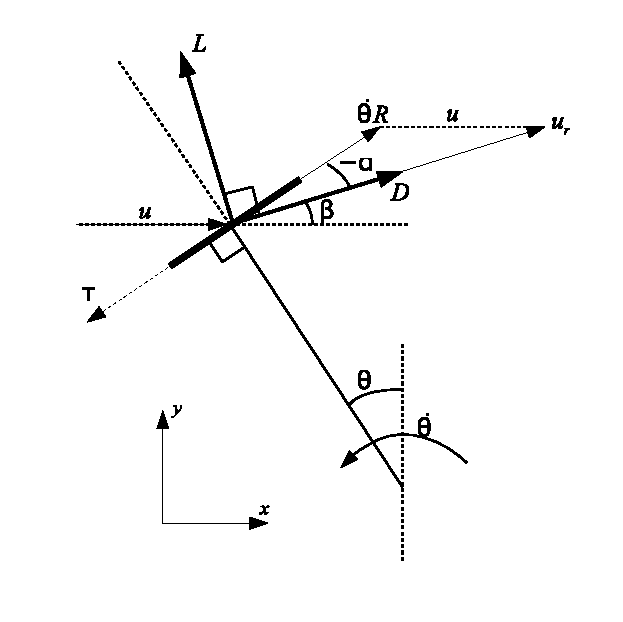
\includegraphics[width=0.7\textwidth]{figuras/EsquemaVelocidade.pdf}
	\fonte{ \citeonline{vallverdu2014}}
	\label{fig:EsquemaVelocidade}
\end{figure}

%Modelo de inclusão de equação. É só copiar, tomar como modelo e modificar.
\begin{equation}
{u_r} = \sqrt {{u^2} + {{(\dot \theta R)}^2} + 2u(\dot \theta R)\cos \theta }
\label{eq:Vrelativa}
\end{equation}

\begin{equation}
\beta  = \arctan \left( {\frac{{\dot \theta Rsen\theta }}{{u + \dot \theta R\cos \theta }}} \right)
\label{eq:beta}
\end{equation}

\begin{equation}
\alpha  = \left| {\frac{{\pi  + \beta  - \theta }}{{2\pi }}} \right| - \pi
\label{eq:alfa}
\end{equation}

Uma vez que o angulo de ataque é conhecido os coeficiente de sustentação ($C_L$) e arrasto ($C_D$) podem ser obtidos. Assim as forças de sustentação ($L$) e arrasto ($D$) podem ser calculadas conforme \autoref{eq:L} e \autoref{eq:D}, respectivamente. Sendo $\rho$ a massa específica do fluido, $c$ a corda, ....

\begin{equation}
L = \frac{1}{2}\rho cu_r^2{C_L}
\label{eq:L}
\end{equation}

\begin{equation}
D = \frac{1}{2}\rho cu_r^2{C_D}
\label{eq:D}
\end{equation}


\section{Modelagem dinâmica}
\label{sec:modelagemdinamica}
